\documentclass[a4paper, 11pt]{article}
\usepackage{geometry}
\usepackage{graphicx}
\usepackage{a4wide}
\usepackage{ulem}
\usepackage{amsthm}
\usepackage{amsmath}
\usepackage{amsfonts}
\usepackage{amssymb}
\usepackage[T1]{fontenc}
\usepackage{ngerman}
\usepackage{graphicx}
\usepackage{epic}
\usepackage{enumerate}
\usepackage{tabu}
\usepackage [latin1]{inputenc}
\geometry{a4paper,left=25mm,right=25mm,top=10mm,bottom=15mm}
%\renewcommand{\baselinestretch}{1.5}
\newcommand{\ol}{\overline}
\newcommand{\makeline}{\hrule\vspace{5pt}}
\newcommand{\ip}[2]{\left< #1, #2 \right>}

\title{3. �bungsblatt zu Software Qualit�t}
\author{Michel Meyer, Manuel Schwarz}

\begin{document}
  \maketitle

  \section*{Aufgabe 3.1}
  \subsection*{(a)}
  \begin{itemize}
    \item{\textbf{Testfall 1:}} zu wenig Geld eingeworfen, min. 1x Geld nachwerfen,
      Getr�nk w�hlen, evtl. R�ckgeld erhalten
    \item{\textbf{Testfall 2:}} zu wenig Geld eingeworfen, Geldr�ckgabehebel ziehen
    \item{\textbf{Testfall 3:}} genug Geld eingeworfen, Geldr�ckgabehebel ziehen
  \end{itemize}

  \subsection*{(b)}
  \subsubsection*{Zust�nde}
  \begin{itemize}
    \item{\textbf{1:}} Bereit
    \item{\textbf{2:}} Geldeinwurf erwarten
    \item{\textbf{3:}} Getr�nkeauswahl erwarten
    \item{\textbf{4:}} Einschenken
    \item{\textbf{5:}} Geld zur�ckgeben
    \item{\textbf{6:}} Fehlverhalten
  \end{itemize}

  \subsubsection*{Aktionen}
  \begin{itemize}
    \item{\textbf{1:}} Geld zwischenlagern
    \item{\textbf{2:}} Geld zur�ckgeben
    \item{\textbf{3:}} Getr�nk ausschenken
  \end{itemize}

  \begin{tabular}[h]{|l|c|c|c|c|c|c|}\hline
                                      & (1)  & (2)  & (3)  & (4)  & (5)  & (6) \\\hline
    Geld einwerfen [Geld $<$ Preis]   & 2 / 1& 2 / 1& 3 /  & 4 /  & 5 /  & 6 / \\\hline
    Geld einwerfen [Geld $\geq$ Preis]& 3 / 1& 3 / 1& 3 / 1& 4 / 1& 5 /  & 6 / \\\hline
    Geldr�ckgabehebel ziehen          & 1 /  & 1 / 2& 1 / 2& 4 /  & 5 /  & 6 / \\\hline
    Getr�nk w�hlen                    & 1 /  & 2 /  & 4 / 3& 4 /  & 5 /  & 6 / \\\hline
    eingeschenkt                      & 6 /  & 6 /  & 6 /  & 5 /  & 6 /  & 6 / \\\hline
    R�ckgeld ausgeben                 & 6 /  & 6 /  & 6 /  & 6 /  & 1 / 2& 6 / \\\hline
  \end{tabular}

  \subsection*{(c)}
  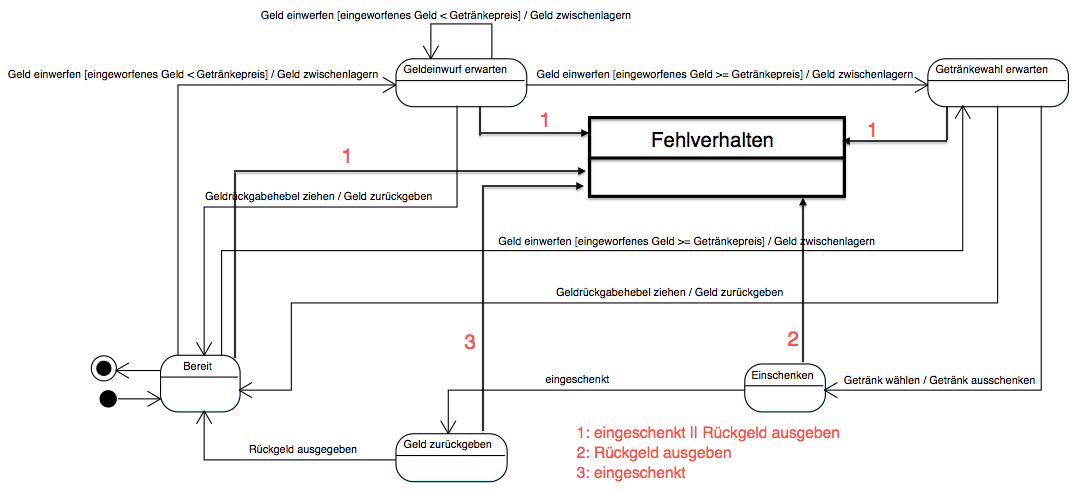
\includegraphics[width=450px]{pictures/aufg3_1.png}

  \section*{Aufgabe 3.2}
  \subsection*{(a) Ursache-Wirkungs-Graph}
  \subsubsection*{Ursachen}
  \begin{itemize}
    \item{\textbf{U1:}} Neukunde
    \item{\textbf{U2:}} auf schwarzer Liste
    \item{\textbf{U3:}} zuverl�ssiger Kunde
  \end{itemize}

  \subsubsection*{Wirkungen}
  \begin{itemize}
    \item{\textbf{W1:}} Kredit ablehnen
    \item{\textbf{W2:}} negatives Anschreiben
    \item{\textbf{W3:}} Kredit bewilligen
    \item{\textbf{W4:}} positives Anschreiben
    \item{\textbf{W5:}} auf schwarzer Liste eintragen
    \item{\textbf{W6:}} Gesch�ftsbeziehung beenden
  \end{itemize}

  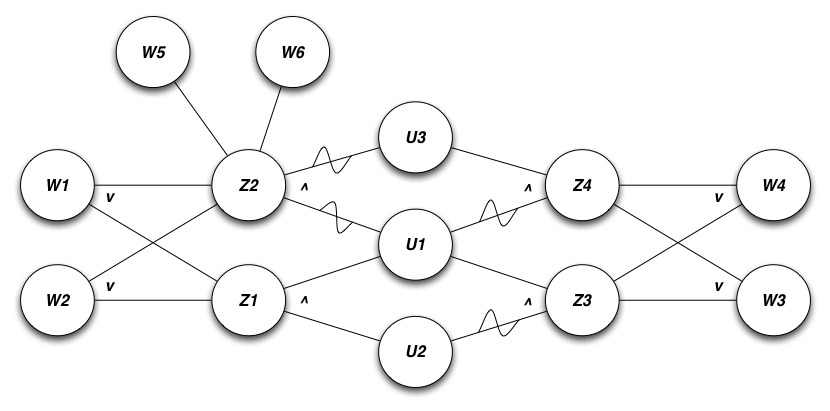
\includegraphics[width=400px]{pictures/aufg3_2.png}

  \subsection*{(b) Entscheidungstabelle}

  \subsubsection*{Beispiel f�r W1:}
  \begin{itemize}
    \item Z1 = 1 oder Z2 = 1
    \item setze Z2 = 1 und Z1 = 0
    \item f�r Z2: U1 = 0 und U3 = 0
    \item f�r Z1: U1 = 0 und U2 = 0
  \end{itemize}
  Eventuell k�nnte man die F�lle in denen U1 = 1 und U3 = 1 sind direkt ignorieren,
  da ein Neukunde kein zuverl�ssiger Kunde sein kann.

  \begin{tabular}[h]{|c||c|c|c|c|c|c|c|c|}\hline
       & 1 & 2 & 3 & 4 & 5 & 6 & 7 & 8 \\\hline\hline
    U1 & 0 & 0 & 0 & 0 & 1 & 1 & 1 & 1 \\\hline
    U2 & 0 & 0 & 1 & 1 & 0 & 0 & 1 & 1 \\\hline
    U3 & 0 & 1 & 0 & 1 & 0 & 1 & 0 & 1 \\\hline\hline
    Z1 & 0 & 0 & 0 & 0 & 0 & 0 & 1 & 1 \\\hline
    Z2 & 1 & 0 & 1 & 0 & 0 & 0 & 0 & 0 \\\hline
    Z3 & 0 & 0 & 0 & 0 & 1 & 1 & 0 & 0 \\\hline
    Z4 & 0 & 1 & 0 & 1 & 0 & 0 & 0 & 0 \\\hline\hline
    W1 & 1 & 0 & 1 & 0 & 0 & 0 & 1 & 1 \\\hline
    W2 & 1 & 0 & 1 & 0 & 0 & 0 & 1 & 1 \\\hline
    W3 & 0 & 1 & 0 & 1 & 1 & 1 & 0 & 0 \\\hline
    W4 & 0 & 1 & 0 & 1 & 1 & 1 & 0 & 0 \\\hline
    W5 & 1 & 0 & 1 & 0 & 0 & 0 & 0 & 0 \\\hline
    W6 & 1 & 0 & 1 & 0 & 0 & 0 & 0 & 0 \\\hline
  \end{tabular}\\
  Aus der obigen Tabelle kann man nun die Spalten 1 und 3, 2 und 4, 5 und 6 sowie 7 und 8
  durch die Optimierung mit Don't Care-Werten (Konsolidierung) zusammenfassen.\\
  Das ergibt dann folgendes Ergebnis (Konsolidierte Entscheidungstabelle):

  \begin{tabular}[h]{|c||c|c|c|c|}\hline
       & 1 & 2 & 3 & 4 \\\hline\hline
    U1 & 0 & 0 & 1 & 1 \\\hline
    U2 & - & - & 0 & 1 \\\hline
    U3 & 0 & 1 & - & - \\\hline\hline
    Z1 & 0 & 0 & 0 & 1 \\\hline
    Z2 & 1 & 0 & 0 & 0 \\\hline
    Z3 & 0 & 0 & 1 & 0 \\\hline
    Z4 & 0 & 1 & 0 & 0 \\\hline\hline
    W1 & 1 & 0 & 0 & 1 \\\hline
    W2 & 1 & 0 & 0 & 1 \\\hline
    W3 & 0 & 1 & 1 & 0 \\\hline
    W4 & 0 & 1 & 1 & 0 \\\hline
    W5 & 1 & 0 & 0 & 0 \\\hline
    W6 & 1 & 0 & 0 & 0 \\\hline
  \end{tabular}

  \section*{Aufgabe 3.3}
  Wird zur Repr�sentation der Fliesenarten eine JAVA-Aufz�hlung (\texttt{enum}) genutzt,
  so k�nnen Testf�lle mit Fliesen aus einem anderen Material als dort definiert sind
  direkt weggelassen werden, da der Test schon im Vorfeld nicht kompilieren w�rde.\\
  Ein solcher Mechanismus wird in der Qualit�tssicherung auch als implizite
  Qualit�tssicherungsma�nahme bezeichnet.


  


\end{document}
